\section{Results}
\label{sec:results}

%\emph{Benchmarks (test results) and possibly competition results.  Include explanations and analyses of your results. As mentioned under “Benchmarks and comparisons” below, it is usually a clear strength if you have some results to com- pare, e.g. two different versions of your client with different methods/features/parameters.  You could also compare the behaviour of your client on different individual levels that illustrate a certain point, e.g. similar levels resulting in large differences in the client’s behaviour.}

This sections presents some results and experiments for our client.
First we present the results of running the competition levels, and then we present an example to illustrate why our goal prioritisation was useful.
Note that we performed our tests on a laptop with Intel® Core™ i5 4210U Processor 2.7 GHz, 4GB DDR3L 1600 MHz SDRAM, with a Solid State Disk.

\Cref{tab:competition results} presents the results of our client on the different levels developed by different groups.
The time is defined in milliseconds, and actions are number of moves performed to solve the level.
The table is split into two columns; one for single-agent levels, and one for multi-agent levels.
There were four levels that were unsolvable, and they are thus ignored.
Our client entered an endless loop for three of the levels (\texttt{SAAIMuffins, SASolo, SABoXBoXBoX}).

It is clear from the results presented in the table, that the client needs improvement because the client crashed for 11 levels (two of which were multi-agent levels).
Our solution did not handle a specific scenario well.
We were not able to locate where the specific problem was.
Moreover, our client was the only client to solve two of the levels (\texttt{MAteamhal, MAAIMuffins}).


\begin{table}
  \centering
  \begin{tabular}{lrrrr}
    \toprule
    \multirow{2}{*}{level creator} & \multicolumn{2}{c}{\underline{single-agent}} & \multicolumn{2}{c}{\underline{multi-agent}} \\
                                   & time & actions & time & actions \\ \midrule
    \texttt{Lazarus}              & 91  & 243 & 62   & 291 \\
    \texttt{Sojourner}            & 144 & 417 & 116  & 255 \\
    \texttt{Optimal}              & 209 & 730 & 161  & 552 \\
    \texttt{DangerBot}            & 402 & 741 & 170  & 716 \\
    \texttt{TheAgency}            & \multicolumn{2}{c}{crash}      & 55   & 39 \\ 
    \texttt{botbot}               & \multicolumn{2}{c}{crash}      & 69   & 87 \\
    \texttt{ButterBot}            & \multicolumn{2}{c}{crash}      & 72   & 175 \\
    \texttt{TheRedDot}            & \multicolumn{2}{c}{crash}      & 123  & 489 \\ 
    \texttt{extra}                & \multicolumn{2}{c}{crash}      & 402  & 1409 \\
    \texttt{teamhal \hfill(!)}    & \multicolumn{2}{c}{crash}      & 334  & 1186 \\ 
    \texttt{AIMuffins \hfill(!)}  & \multicolumn{2}{c}{live-lock}  & 3695 & 1417 \\ 
    \texttt{WallE}                & \multicolumn{2}{c}{unsolvable} & 157  & 506 \\
    \texttt{FortyTwo}             & \multicolumn{2}{c}{crash}      & \multicolumn{2}{c}{unsolvable} \\
    \texttt{NoOp}                 & \multicolumn{2}{c}{crash}      & \multicolumn{2}{c}{unsolvable} \\
    \texttt{TAIM}                 & \multicolumn{2}{c}{crash}      & \multicolumn{2}{c}{unsolvable} \\
    \texttt{Solo}                 & \multicolumn{2}{c}{live-lock}  & \multicolumn{2}{c}{crash}      \\
    \texttt{BoXBoXBoX}            & \multicolumn{2}{c}{live-lock}  & \multicolumn{2}{c}{crash}      \\
    \bottomrule
  \end{tabular}
  \caption{\label{tab:competition results}The stats of our client's solutions for the different levels. The exclamation mark \texttt{(!)} defines levels that only our client solved.}
\end{table}


\subsection{Different Goal Prioritisations}

To showcase how efficient our goal prioritisation technique was and how we have improved upon it throughout the project, we present some test runs using the \texttt{SAOptimal} level. 
We have chosen this level, as it requires a good goal prioritisation in order to solve efficiently.
In the following we will refer to our main goal prioritisation technique (\cref{methods:goal_ordering}) as the ``complex'' prioritisation, and use the term ``simple'' to mean a prioritisation that does not require a strict ordering of grouped goals, as presented in \cref{methods:goal_ordering} (the second step).
The intuition is that goals placed in dead-ends or corners must be achieved before any goals that would otherwise block the path to the inner most goals.

We illustrate three runs on the same level; 
one with no goal prioritisation whatsoever (\cref{fig:no priority}),
one with simple goal prioritisation (\cref{fig:simple priority}), and 
one with complex goal prioritisation (\cref{fig:complex_priority}). 

% Example of cells
\begin{figure}[h!]
  \centering
  \begin{minipage}{.30\columnwidth}
    \centering
    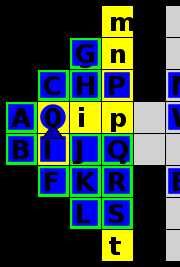
\includegraphics[height=3cm]{graphics/no_priority_block.png}
    \caption{\label{fig:no priority}Arbi\-tra\-ry prioritisation.}
  \end{minipage}%
  \hspace{10pt}%
  \begin{minipage}{.30\columnwidth}
    \centering
    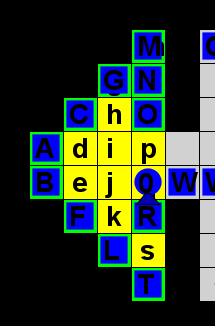
\includegraphics[height=3cm]{graphics/simple_priority_block.PNG}
    \caption{\label{fig:simple priority}Simple prioritisation.}
  \end{minipage}%
  \hspace{10pt}%
  \begin{minipage}{.30\columnwidth}
    \centering
    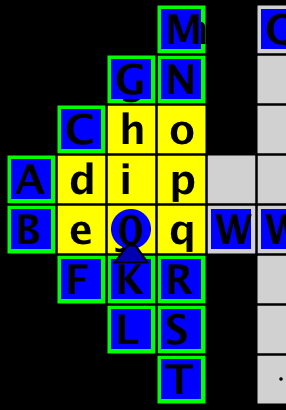
\includegraphics[height=3cm]{graphics/complex_priority.png}
    \caption{\label{fig:complex_priority}Comp\-lex prioritisation.}
  \end{minipage}
\end{figure}

The main difference between the complex and simple prioritisation is that the complex forces a specific order on goals which are grouped, as mentioned in \cref{methods:goal_ordering}.
As \cref{fig:complex_priority} illustrates the complex prioritisation results in the goals next to the level's bounds to be fulfilled first. 
The lack of strict order for the simple prioritisation (as illustrated in \cref{fig:simple priority}) results in the agent choosing to place \textbf{R} before \textbf{S} and thus blocking the path of a goal (the priority of these two boxes is the same in the example, because they have the same number of walls, goals, and free neighbour cells).
With arbitrary prioritisation (as presented in \cref{fig:no priority}) even more goals are blocked by the fulfilment of others.

Our final client utilized the complex prioritisation method, and with this we managed to solve this level (\texttt{SAOptimal}) with 31 fewer actions than the simple prioritisation as presented in \cref{tab:SAOptimal_results}.

\begin{table}[h!]
  \centering
  \begin{tabular}{@{}ll@{}}
    \toprule
    Prioritisation technique & Actions \\
    \midrule
    None    & $>1000$ \\
    Simple  & $761$ \\
    Complex & $730$ \\
    \bottomrule
  \end{tabular}
  \caption{\label{tab:SAOptimal_results}No. actions performed on \texttt{SAOptimal} level with different prioritisation techniques.}
\end{table}

We found that a client with no goal prioritisation requires almost 50 \% more actions on this level than with some kind of prioritisation technique.
This is due to the fact that many actions are wasted because the inner most goals are left open, and thus as the client wants to achieve them, all the previous boxes must be moved.

\subsection{Performance vs. Optimality}
\label{sec:performance vs. optimality}

We have developed a client with simplicity in mind.
The only technique we used to yield more intuitive solutions was to develop the goal prioritisation technique, so the client did not fill in goals arbitrarily.
From the course's competition presentation we found that, as an example, our client was beaten in \texttt{SAOptimal} with about 7 \% less actions performed.
However, our client solved the level approximately 700 times faster than the opponent.\footnote{\textbf{opponent}: $143{,}297$ ms with $680$ actions \& \textbf{our}: $209$ ms with $730$ actions. (source: competition results)}
We presented our client's statistics in \cref{tab:competition results}, and the level mentioned here was created by \texttt{Optimal} for single-agent movement.

\subsection{Multi-agent and Single-agent Levels}

Though the level \texttt{SAOptimal} showcases the importance of some goal prioritisation, it is important to note that out of the 16 levels we managed to solve, most of them were multi-agent levels. For the multi-agent levels, we only move one agent at a time and therefore lose a lot of performance w.r.t. the number of actions performed. 
On the time performance however, again here we perform very well as with the single-agent levels. 
As presented in \cref{tab:competition results} our client was able to solve most of the multi-agent levels.
